\documentclass[a4paper,12pt]{article}

\usepackage[utf8]{inputenc}
\usepackage[T1]{fontenc}
\usepackage{graphicx}
\usepackage{color}
\usepackage{amsmath}
\usepackage{amsfonts}
\usepackage{amssymb}
\usepackage{multicol}
\usepackage{eurosym}
\usepackage{bbm}
\usepackage[french]{babel}
\usepackage{lastpage}
\usepackage{float}
\usepackage{upgreek}
\usepackage{verbatim}
\usepackage{moreverb}
\usepackage{listings}
\usepackage{textcomp}
\usepackage[nottoc]{tocbibind}
\usepackage{hyperref}
%\usepackage{subfigure}
\usepackage{subcaption}
\usepackage{ulem}
\usepackage{etoolbox}

\usepackage{colortbl}
\usepackage{xcolor}

\definecolor{color_caption}{rgb}{0.3,0.3,0.3}
\definecolor{color_section}{rgb}{0.9,0,0}
\definecolor{em_orange}{rgb}{0.9686,0.5765,0.1137}
\definecolor{em_pink}{rgb}{0.9294,0.0078,0.5490}
\definecolor{em_blue}{rgb}{0.1412,0.6667,0.8824}
\definecolor{em_green}{rgb}{0.5451,0.7765,0.2431}

\usepackage{caption}
\usepackage[font={color=color_caption},figurename=Figure,labelfont={it}]{caption}

\lstset{
language=C,basicstyle=\normalsize,upquote=true,aboveskip={1.5\baselineskip},columns=fullflexible,showstringspaces=false,extendedchars=true,breaklines=true,showtabs=false,showspaces=false,showstringspaces=false,identifierstyle=\ttfamily,keywordstyle=\color[rgb]{0,0,1},commentstyle=\color[rgb]{0.133,0.545,0.133},stringstyle=\color[rgb]{0.627,0.126,0.941},}

\DeclareMathOperator{\G}{G}

\renewcommand{\arraystretch}{1.5}
\renewcommand{\baselinestretch}{1.5}

\textheight 255mm
\headheight 15mm
\oddsidemargin -10mm
\evensidemargin -10mm
\marginparwidth 5mm
\topmargin -20mm
\textwidth 185mm
\headsep 5mm
\footskip 10mm


\usepackage{fancyhdr}

\pagestyle{fancy}

\renewcommand{\headrulewidth}{2pt}
\renewcommand{\headrule}{\hbox to\headwidth{\color{em_orange}\leaders\hrule height \headrulewidth\hfill}}
\fancyhead[L]{ENSEIRB-MATMECA}
\fancyhead[C]{Projet avancé SE}
\fancyhead[R]{E3}

\renewcommand{\footrulewidth}{2pt}
\patchcmd{\footrule}{\hrule}{\color{em_orange}\hrule}{}{}
\fancyfoot[C]{\thepage}

\usepackage{eso-pic}
\newcommand\BackgroundPic{%
\put(0,0){%
\parbox[b][\paperheight]{\paperwidth}{%
\vfill
\centering

\includegraphics[scale=0.6,%
keepaspectratio]{background}%
\vfill
}}}


\begin{document}
\parindent=1cm
\everymath{\displaystyle}
%
\AddToShipoutPicture*{\BackgroundPic}
%
\thispagestyle{empty}
%
%
\noindent
Cédric DUMONDELLE\hfill{E3}\\
Lucas FILLON\\
Xavier MARINO\\
Pierre OLIVIER\\
%
\\
%
\vspace{5.5cm}
{\color{white}t}\\
%
{\color{em_orange}\rule{\linewidth}{2pt}}
%
\textbf{{
\begin{center}
\Huge Projet avancé SE\\
%\vspace{0.6cm}
\end{center}
}}
%
{\color{white}t}\\
{\color{em_orange}\rule{\linewidth}{2pt}}\\

\vspace{9.5cm}

%
Yannick BORNAT \& Bertrand LE GAL
% \begin{tabular}{rcl}
% Dominique Dallet\hspace{4cm}\vphantom{e}&
% Professor Izzet Kale\hspace{4cm}\vphantom{e}&
% Saumya Reni
% \end{tabular}
% %
\ClearShipoutPicture
%
\newpage
%
\thispagestyle{empty}
\tableofcontents
%
\newpage
%%%%%%%%%%%%%%%%%%%%%%%%%%%%%%%%%%%%%%%%%%%%%%%%%%%%%
\setcounter{section}{-1}
\section{Introduction}
\subsection{Contexte}
De nos jours, nous disposons de différents moyens de conception, tous proposant des avantages et des inconvénients. Certains sont plus simple à mettre en œuvre, d'autres sont plus complexe mais sont généralement la solution la plus efficace. Il faut toujours mesurer le besoin d'un projet pour choisir correctement la voie de développement à privilégier.
On peut globalement résumer les différents moyens de conception en quatre grandes familles, respectivement ordonnées de la plus souple à la plus rigide, de la plus généraliste à la plus spécifique: CPU, GPU, FPGA, ASIC. Cependant ces quatre familles peuvent être réunies en deux grandes familles: les solutions \textit{software} (CPU, GPU) et les solutions \textit{hardware} (FPGA, ASIC).
Dans un projet, il existe de nombreuses contraintes, qu'elles soient temporelles, financières, juridiques, humaines, etc. Ces contraintes ne sont pas négligeables, d'autant plus à échelle industrielle ou gouvernementale où la taille des projets et les moyens investis peuvent être considérables, par conséquent il est important de bien juger de la direction à prendre dans le projet pour éviter un gaspillage de ressources. \newline
\begin{comment}a propos du terme gouvernementale : les projets type gouvernementaux ou mondiaux comme la conception d'un télescope, d'une fusée, d'une station spatiale, d'un rover martien, des projets massif mais presque unique qui sont pas a visé d'un industrialisé \end{comment}

Les solutions \textit{software} permettent un développement rapide, souple, peu coûteux et adaptable à de nombreuses situations cependant elles peuvent être insuffisamment efficace dans certains cas. En effet certains systèmes demanderont une réactivité bien plus grande, une consommation énergétique bien plus faible voir une consommation matérielle limitée. Pour répondre à ces contraintes l'utilisation des solutions dites \textit{hardware} est préférable. Les FPGA et les ASIC permettent l'implémentation \textit{hardware} de fonctions logiques spécifiques, ainsi leurs performances seront sensiblement meilleures pour la plupart des projets. En effet les solutions \textit{hardware} permettent généralement de diminuer le coût énergétique du projet en n'implémentant que les fonctions dont on a besoin, et pour la même raison, d'augmenter l'efficacité du système pour une tâche donnée, elles permettent même de réduire le coût silicium dans le cadre de l'ASIC. Cependant l'implémentation \textit{hardware} fige l'utilisation de ces solutions à un seul et unique usage et ces solutions sont souvent coûteuses en termes de temps et de frais de développement.\newline


La technologie FPGA pour \textit{Field Programmable Gate Array} consiste en un large réseau de portes logiques, de petites mémoires appelées LUT, de bascules, qui peuvent être connectées entre elles, comme on le souhaite, afin de réaliser des fonctions logiques plus ou moins complexe. La technologie FPGA est donc avantageuse car un FPGA est entièrement configurable, performant et peu coûteux lorsqu'on ne souhaite pas produire de grandes quantités. Le FPGA est plus intéressant que les solutions \textit{software} pour effectuer des tâches complexes particulières et plus intéressant que l'ASIC d'un point de vue temps et coûts de développement.\newline 

Pour configurer un FPGA, différents langages ont été développés permettant de décrire les fonctions logiques que l'on souhaite implémenter dans le FPGA. Celui qui nous intéresse se nomme le VHDL mais le principe est similaire avec les autres langages de la même famille tel que le Verilog. Le VHDL est donc un langage de description, c'est à dire que l'outil de synthèse câblera le FPGA comme le VHDL le décrit. Le niveau d'abstraction est très faible, ce qui signifie qu'il est nécessaire de s'assurer de la synchronisation entre les différentes étapes d'un \textit{process}, du bon dimensionnement des données, de gérer les cas particuliers d'une opération... Ce niveau d'abstraction permet une précision chirurgicale très intéressante pour des petits systèmes mais qui peut vite devenir complexe lorsque le projet devient important. Les principaux défauts de ce langage sont les suivants :
\begin{itemize}
\item[•] Il est complexe à appréhender, notamment pour des programmeurs;
\item[•] Il est élitiste, peu de personnes le onnaissent et sont à l'aise avec ce langage;
\item[•] Il est exigeant, une erreur dans la description et la synthèse peut donner un résultat non fonctionnel difficile à corriger;
\item[•] Une description fonctionnelle est difficile à modifier sans créer de nouvelles erreurs et sans perdre de temps.
\end{itemize}

Au début les langages HDL, \textit{Hardware Decription Language}, tel que le VHDL était la seule solution pour développer sur FPGA, mais depuis une dizaine d'années un nouveau langage est apparu : le SystemC. La taille des FPGA est devenue vraiment importante par conséquent les projets devinrent important eux aussi. Il devenu courant de parler d'implémentation sur FPGA de processeurs \textit{softcore}, de décodeurs vidéos multi-formats, de récepteurs ethernet. Mais avec le VHDL, il devient très vite fastidieux de développer de tels projets, c'est dans ce but que le SystemC à été créé. Le principe étant de réduire le temps de développement en proposant un niveau d'abstraction plus haut que le VHDL. Ainsi il est possible de décrire du \textit{hardware} tout en faisant abstraction de notions très bas niveau. C'est un langage basé sur le C++ donc plus simple à appréhender pour des programmeurs, des informaticiens ou des {\color{red}traiteurs du signal} travaillant à haut niveau, permettant ainsi à ces derniers de travailler sur les mêmes sources que les électroniciens, ce qui rompt l'élitisme du VHDL. La nature haut niveau et orientée objet de ce langage le rend également plus flexible et plus facile à corriger. De plus les différents niveaux d'abstractions apportés par les nombreux types du SystemC permettent de simuler rapidement un concept puis de l'affiner par la suite. Évidemment on perd la maîtrise sur la synthèse et il devient difficile de savoir comment l'outil a synthétisé notre système. On perd également en contrôle sur l'optimisation, le SystemC ne permettant pas d'être aussi précis que le VHDL mais il est possible de s'y approcher. 

\subsection{Problématique}

Certaines différences entre le VHDL et le SystemC ont été mises en évidence dans la partie précédente mais ces différences sont spéculatives. Les portraits dressés du SystemC et du VHDL semble montrer que ce dernier est obsolète pour les nouveaux projets qui se développe sur FPGA et que le SystemC est un outil plus approprié et puissant. Le but de ce projet est de confronter ces deux portraits à la réalité grâce au développement d'un projet VHDL et en SystemC, puis d'étudier la finalité de ces deux projets.\newline

Notre problématique sera donc la suivante : Quel sont les avantages du SystemC par rapport au VHDL dans le développement d'un système complexe ?  
Que permet l’utilisation du systemC par rapport au VHDL dans le cadre du développement d’un système complexe ? \newline
% Faut fixer une probl"matique !!
Ainsi nous allons chercher à comparer les possibilités que le SystemC nous apporte par rapport au VHDL. Un projet a déjà été developpé et implémenté en VHDL par monsieur Bornat. Ce projet consiste en une chaîne de traitement de signaux biologiques permettant de détecter l'activité de cellules organiques. Nous allons développer cette même chaîne de traitement grâce au SystemC mais nous allons également développer une variante de ce projet. En effet il existe deux méthodes pour calculer le seuil permettant de détecter l'activité des cellules qui seront présentées plus tard dans ce rapport.\newline
Dans la partie suivante, l'architecture de la chaine de traitement sera présentée en détail avec les étapes de \textit{process} et la répartition des tâches sous forme de blocs. L'implémentation en SystemC fera l'objet de la troisième partie en commençant par décrire le flot de conception d'un projet utilisant le SystemC, puis la manière dont le projet a été décrit en SystemC et simulé afin de valider les sources, et enfin en finissant par l'implémentation sur le FPGA, les problèmes que l'implémentation a posé et la manière dont elle a été validé. Dans la quatrième partie nous interpréterons les résultats d'un point de vue technique mais également humain. Ce rapport se terminera avec une cinquème et dernière partie qui fait office de conclusion.

\newpage
\section{Présentation du cas d'étude}
\subsection{Introduction}
Afin de mener à bien cette étude nous nous sommes basés sur les travaux de Yannick Bornat. En effet, dans le cadre de l'analyse de signaux biomédicaux, ce dernier a mis au point un module de détection d'activité de cellules biologiques, en VHDL.\\

Dans le cas de signaux provenant de cellules biologiques, l'activité cellulaire peut être détectée par un pic d'amplitude, celui-ci est représenté en figure 1. Cependant ce type de signaux possède une composante en bruit basse fréquence très élevée, c'est pourquoi il doit être filtré en amont. C'est ce signal filtré qui est utilisé à la détermination d'une valeur de seuil nécessaire à la détection d'activité biologique. Ce principe de fonctionnement, qui sera à la base du développement de notre module, est illustré en figure 2.\\

\begin{figure}[H]
\centering
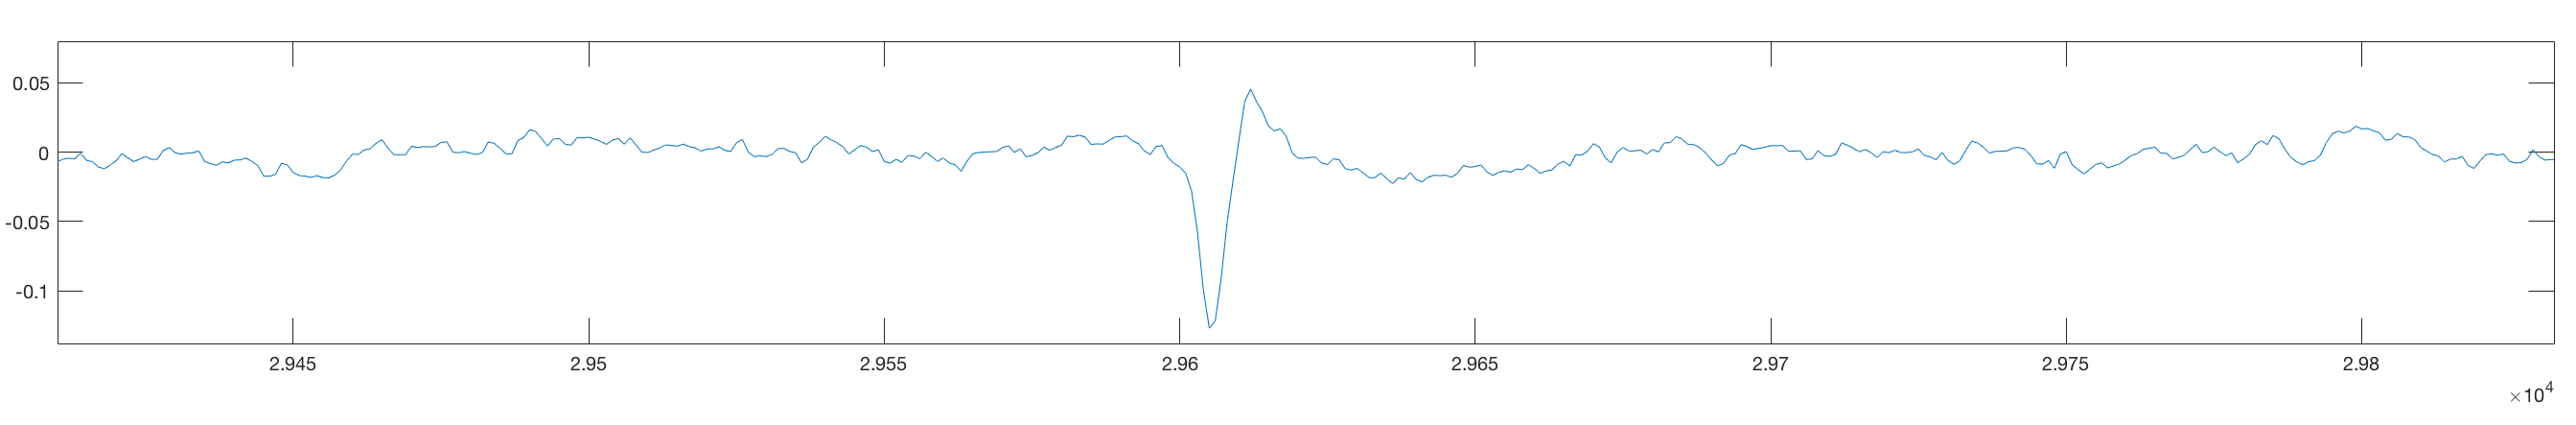
\includegraphics[scale=0.18, keepaspectratio]{toto3.png}
\caption{\textit{Pic d'activité dans un signal biologique}}
\end{figure}

\begin{figure}[H]
\centering
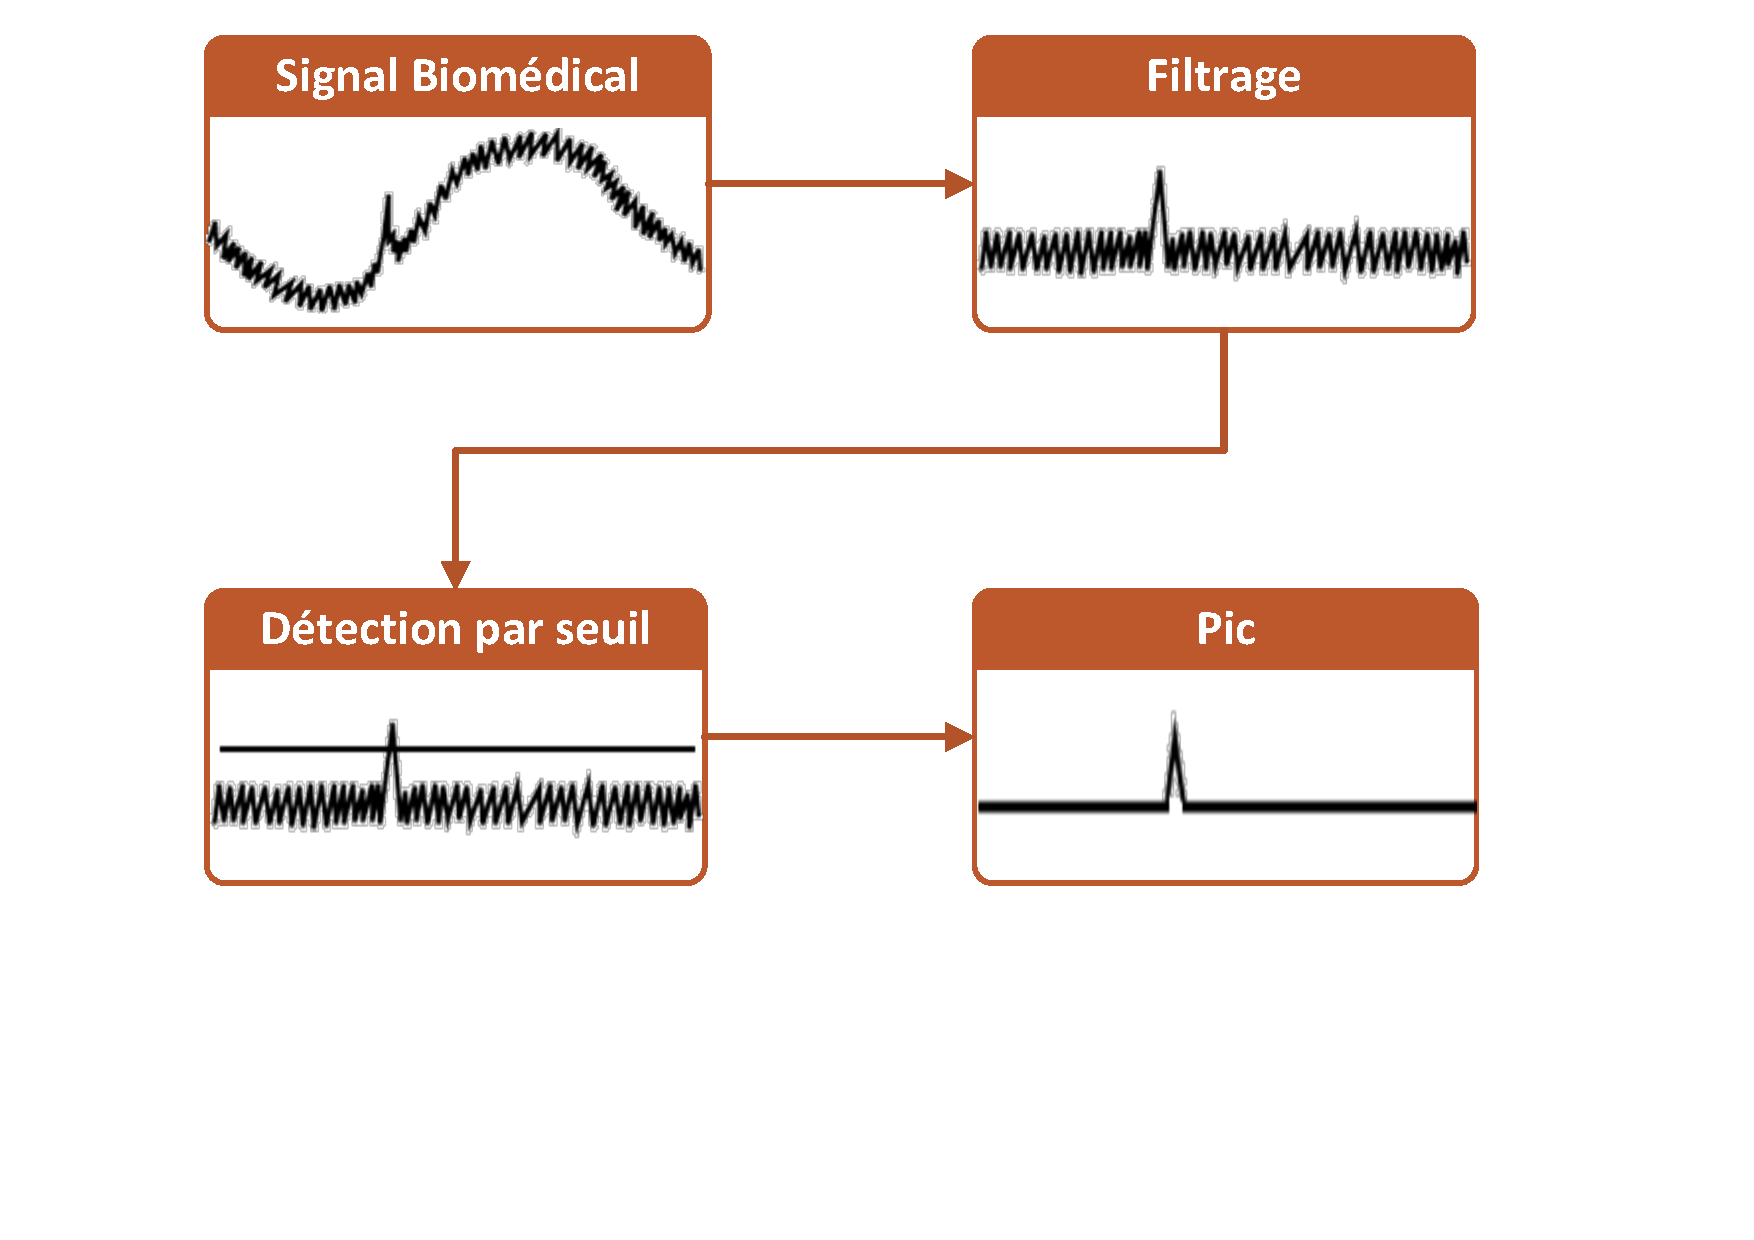
\includegraphics[scale=0.5, keepaspectratio]{Dessin1.pdf}
\caption{\textit{Principe de fonctionnement du module de détection d'activité cellulaire}}
\end{figure}
\newpage

\subsection{Fonctionnement des différents blocs}
Comme énoncé précédement, les signaux issus de capteurs biologiques sont très fortement bruité en basse fréquence, ceci se caractérise par une forte variation de l'amplitude du signal. Cette variation d'amplitude, illustrée en figure 3 a) sur 5000 échantillons, est du même ordre, voir plus grand, que les pics attestant d'une activité celllulaire. Il convient donc de supprimer ce bruit afin de correctement détecter les pics d'activité.\\

\begin{figure}[H]
\centering
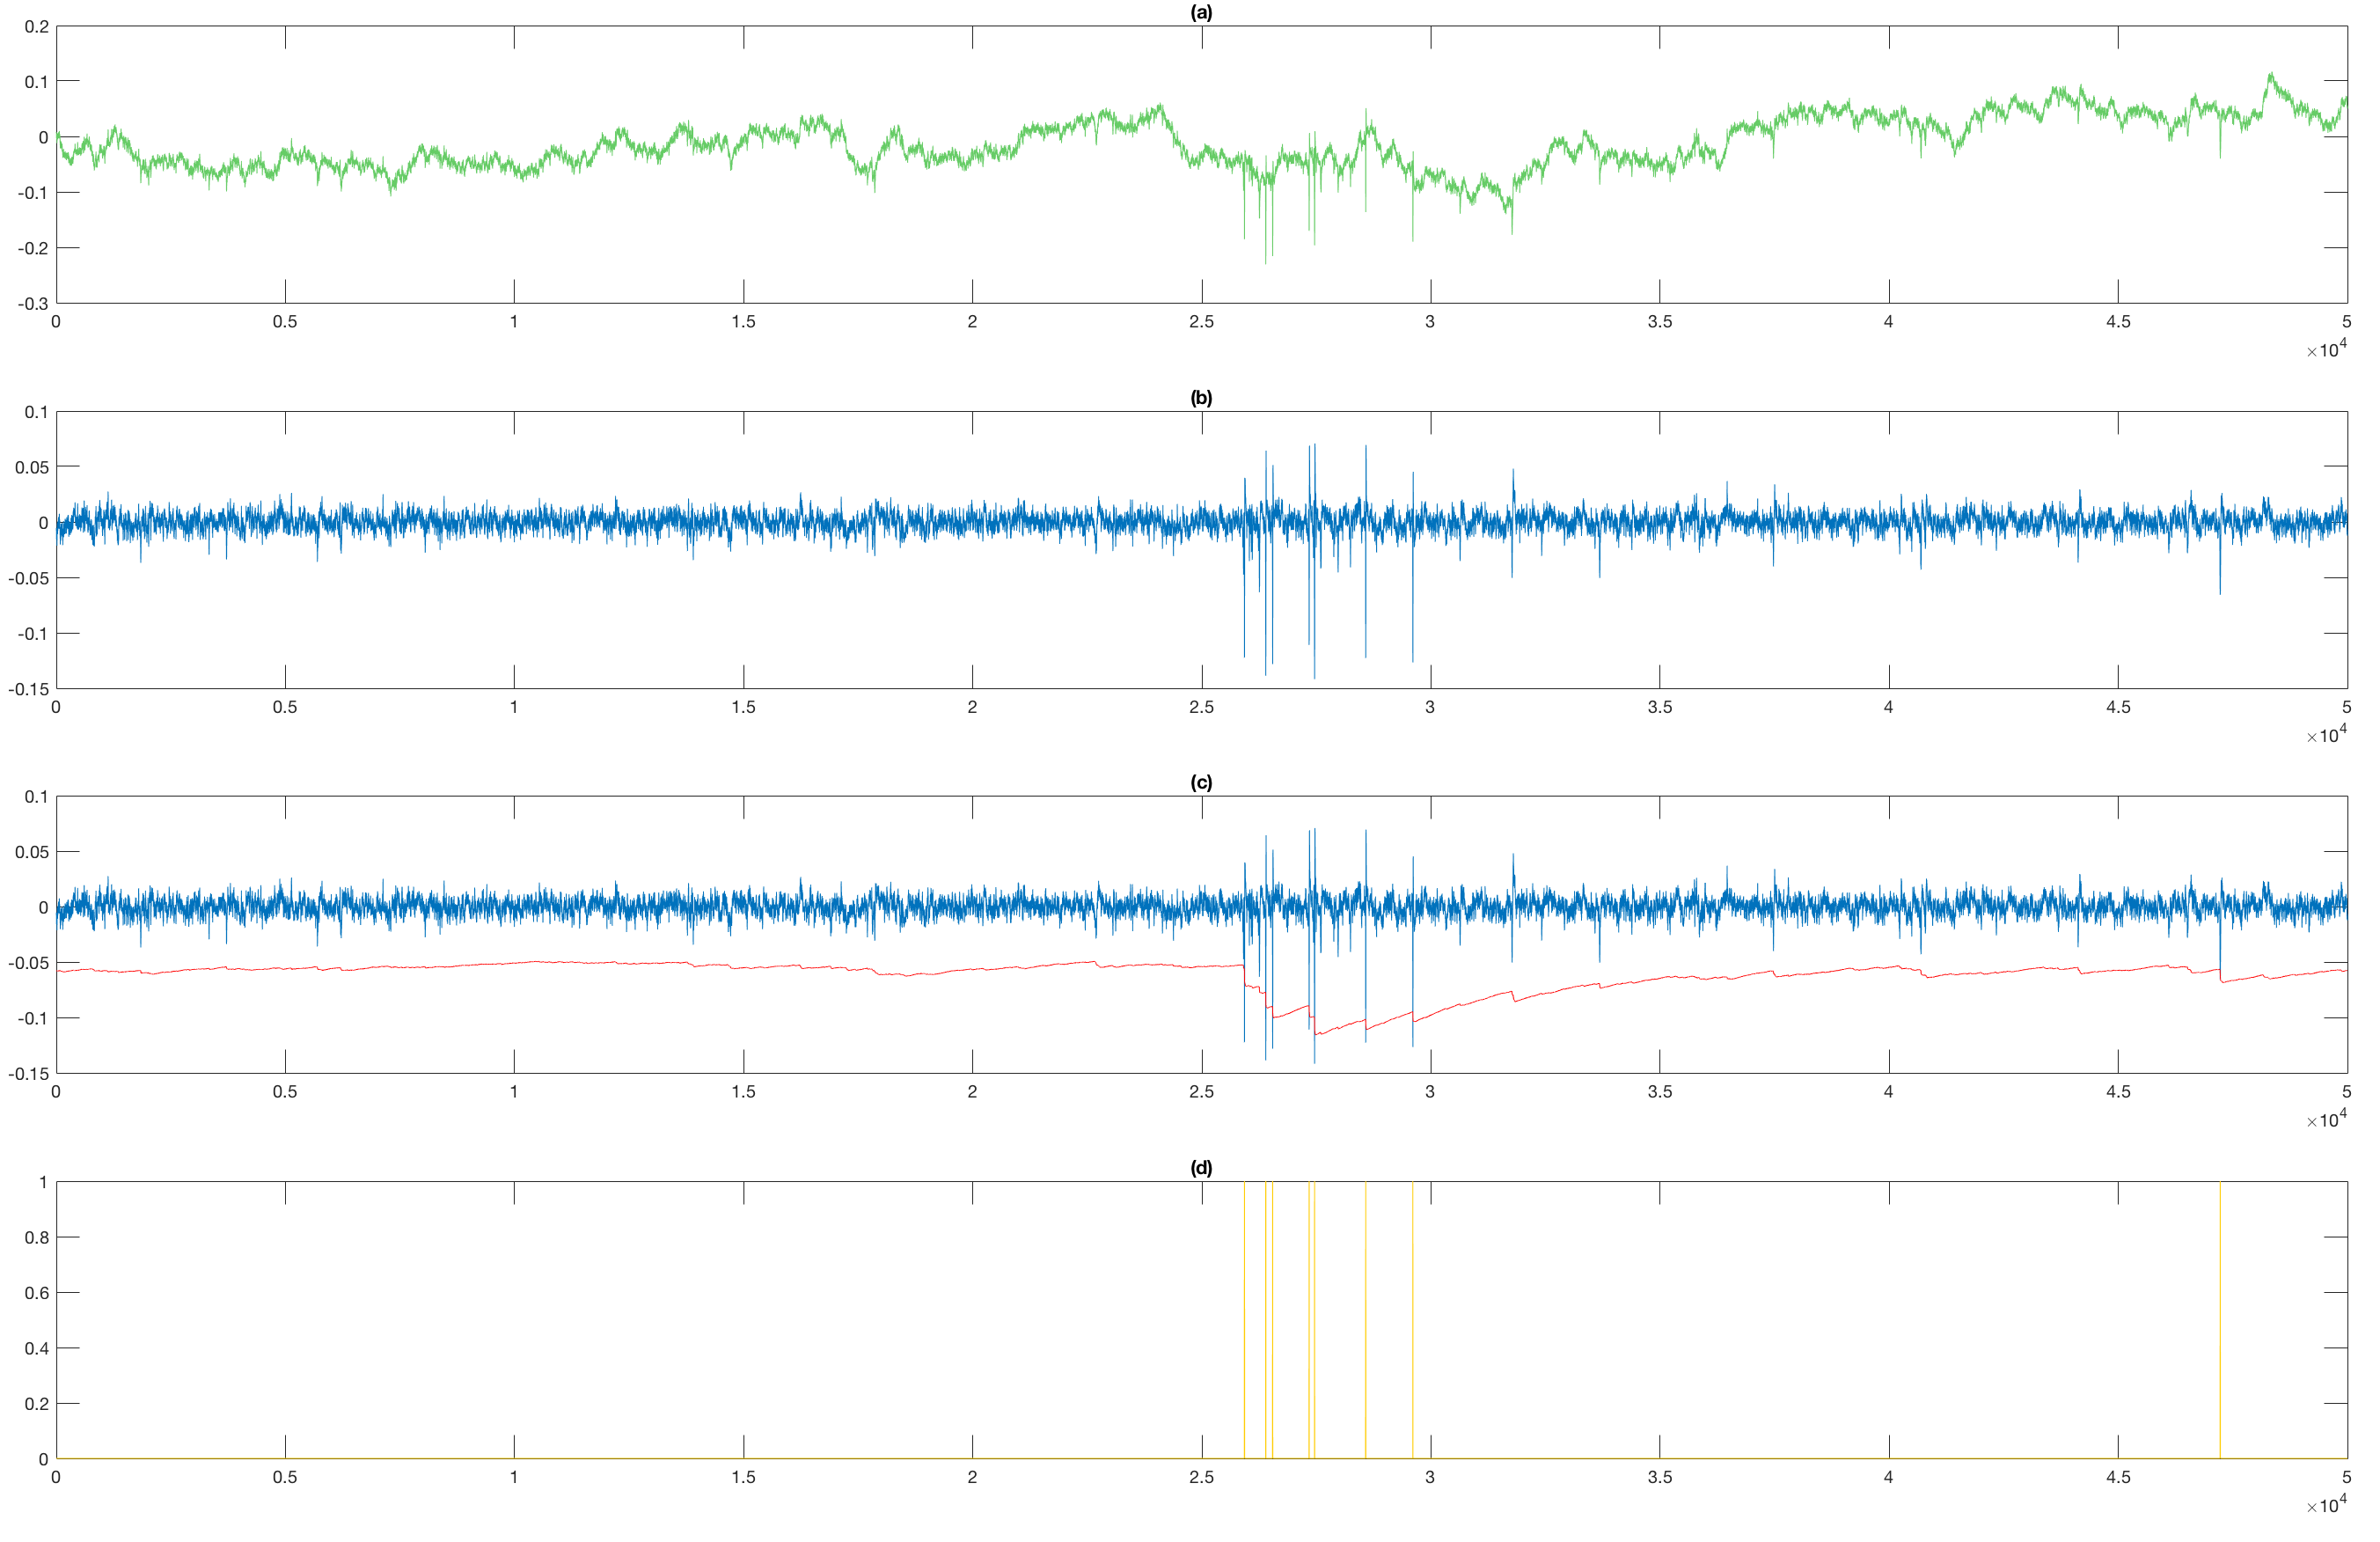
\includegraphics[scale=0.18, keepaspectratio]{toto2.png}
\caption{\textit{Évolution du signal au cours des différentes étapes de filtrage, sur 5000 échantillons}}
\end{figure}

\begin{itemize}
\item[•] \textbf{Suppression du bruit basse fréquence contenu dans le signal d'entré} : c'est un filtre passe-haut à réponse impulsionnelle infinie (IIR) qui est utilisé pour s'affranchir des basses fréquence, suivant l'équation (1).
\begin{eqnarray}
y_n = \frac{63}{64}\left(x_n - x_{n-1}\right) + \frac{31}{32}y_{n-1}
\end{eqnarray}
Le résultat issus de cette première étape de filtrage est illustré en figure 3 b), on retrouve les pics caractéristiques du signal, mais celui-ci est désormais centré sur 0. On peut, cependant, constater que ce signal est également bruité en haute fréquence. C'est pour limiter l'impact de ce bruit, qu'une valeur de seuil adaptative est utilisée afin détecter les pics.\\

\item[•] \textbf{Calcul de la valeur de seuil} : deux modèles différents ont été explorés lors de cette étape, l'un d'entre eux reprennant les travaux de Yannick Bornat en appliquant une boucle de correction sur le signal d'entré filtré, tandis que l'autre méthode utilise la valeur d'écart type, de nouveau appliqué au signal filtré, (à un facteur de proportionnalité près), comme valeur de seuil.\\

\begin{itemize}
\item[\textbf{a)}] \textbf{Calcul du seuil par boucle de correction} :
\begin{figure}[H]
\centering
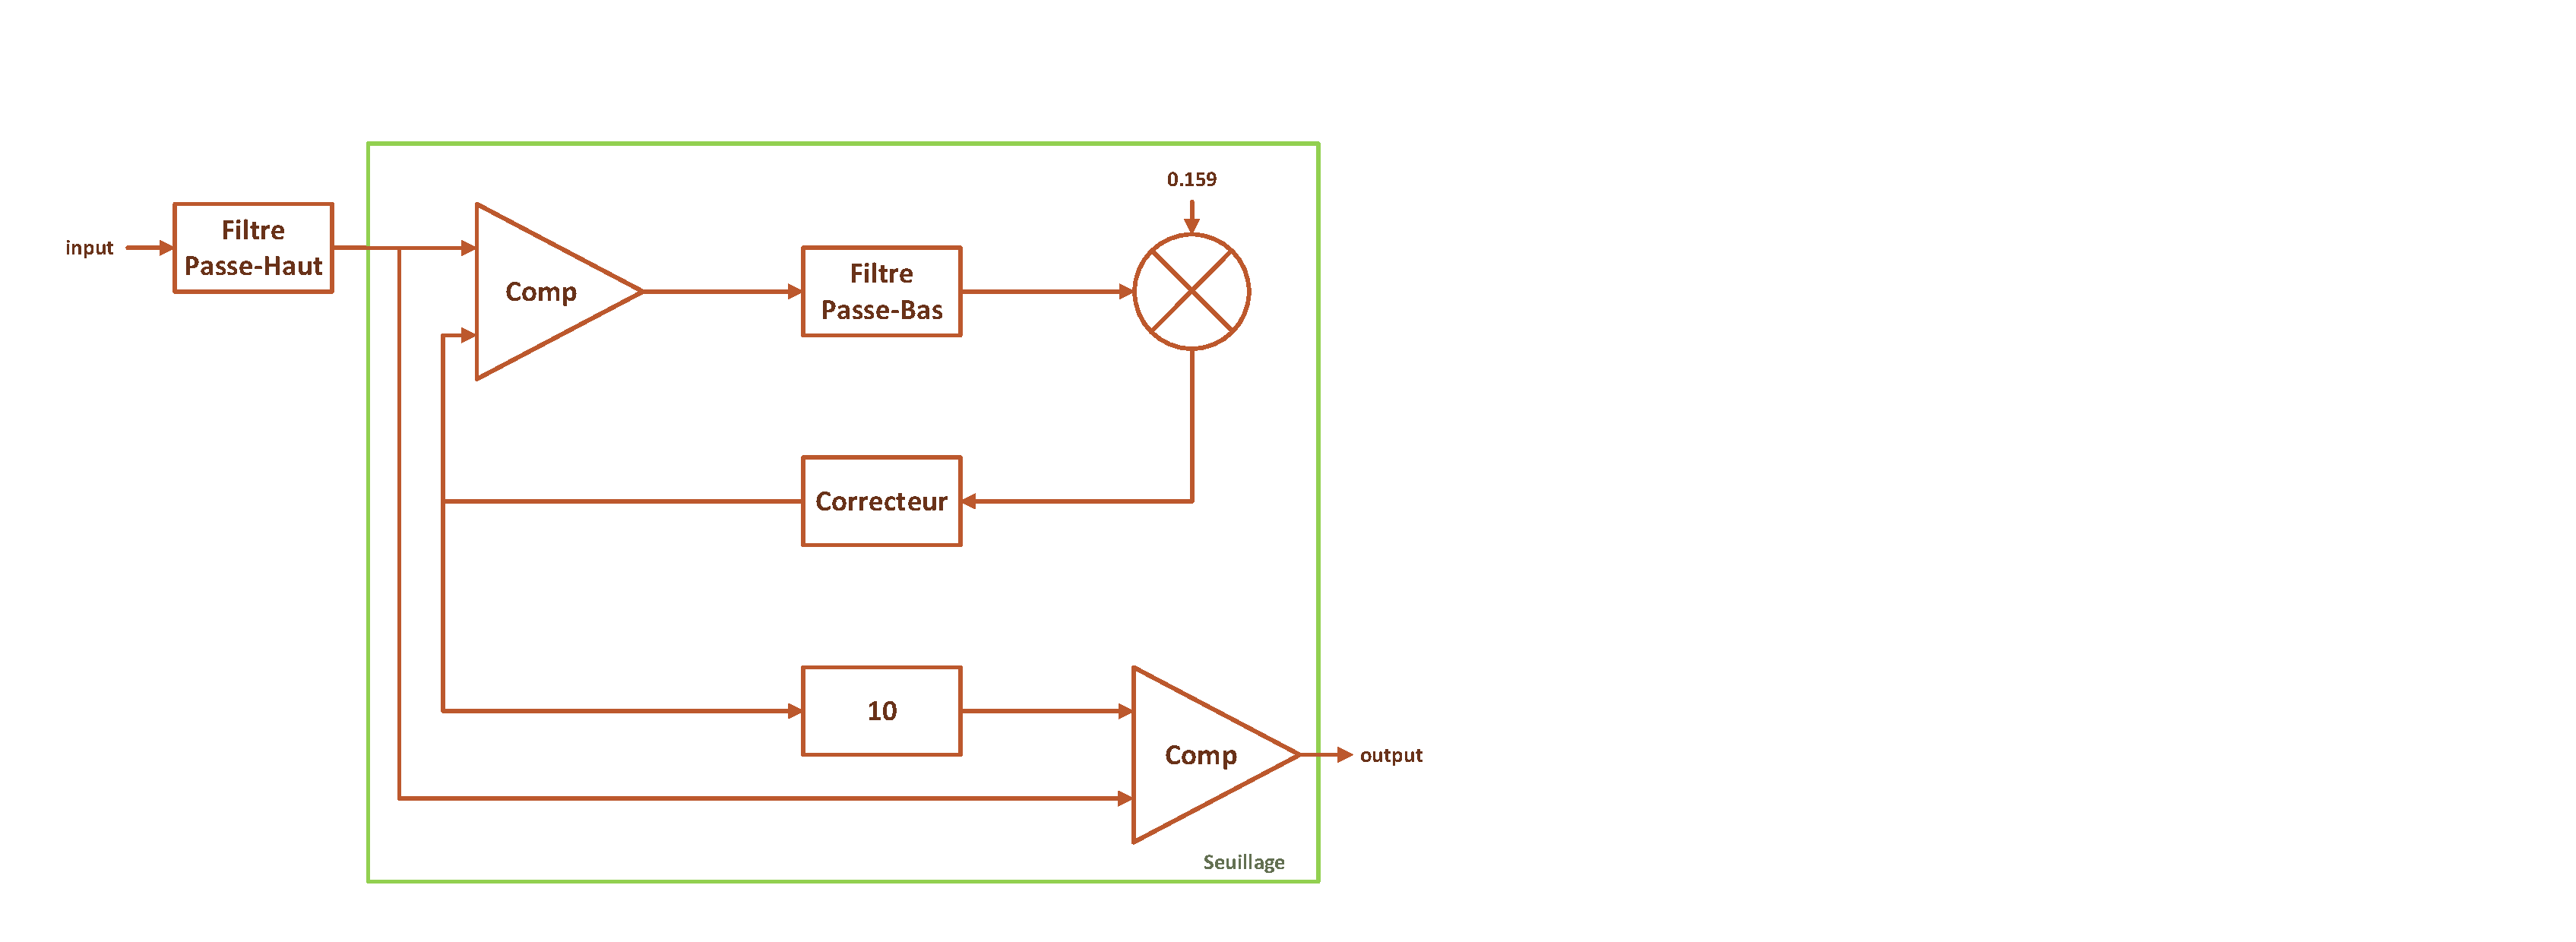
\includegraphics[width=\textwidth, keepaspectratio]{chainCedric.pdf}
\caption{Architecture du seuillage avec correcteur}
\end{figure}
Dans ce modèle dont l'architecture est représentée figure 4, le but est de fixer le seuil de façon à ce qu'uniquement $15.9 \%$ des échantillons soient supérieurs à celui-ci. Dans ce but, une boucle de contre-réaction est mise en place afin d'adapter la valeur de seuil afin de remplir cette condition. Dans un premier temps, l'échantillon est comparé avec la valeur de seuil actuelle. Le comparateur produira un niveau haut si celui-ci est supérieur au seuil et produira un niveau bas sinon. Le filtre passe-bas qui suit sert de moyenneur. En effet, celui-ci permet de calculer la valeur moyenne des sorties du comparateur sur un certain nombre d'échantillons. En d'autres termes, il donne en sortie le pourcentage d'échantillon au-dessus de la valeur de seuil. Après soustraction de $0.159$, la valeur de sortie de ce moyenneur est envoyé en entrée du correcteur composé d'un proportionnel intégrateur ce qui permet d'annuler l'erreur statique. Cette boucle de contre-réaction permet la mise à jour perpétuelle de la valeur de seuil. Pour finir, les échantillons sont comparés à celle-ci multiplié par $10$ et le résultat de cette comparaison est envoyé en sortie. Ce résultat correspond à la présence (niveau haut) ou non (niveau bas) d'un pic.
\item[\textbf{b)}] \textbf{Calcul du seuil par écart type} : dans cette méthode, le calcul de la valeur de seuil est assimilé au calcul de l'écart type du signal d'entré filtré. On a donc, pour une distribution uniforme des échantillons :
\begin{eqnarray*}
S = \sqrt{\frac{\sum^N_{i=1}\left(x_i-\overline{x}\right)^2}{N}},
\end{eqnarray*}
or dans notre, comme il a été souligné plus tôt, la valeur moyenne du signal a été ramenée à 0 grâce à la première étape de filtrage, on obtient donc :
\begin{eqnarray*}
S = \sqrt{\frac{\sum^N_{i=1}x_i^2}{N}}.
\end{eqnarray*}
Enfin, la fonction $x_n\mapsto\frac{\sum^N_{i=1}x_i}{N}$ a été réalisé à l'aide d'un filtre passe-bas à réponse impulsionnelle infinie, suivant l'équation (2). Les facteurs de ce filtre ont été dimensionnés afin de cibler le bruit en haute fréquence du signal.
\begin{eqnarray}
y_n = \frac{1}{524288}\left(x_n + x_{n-1}\right) + \frac{2047}{2048}y_{n-1}
\end{eqnarray}
La valeur de seuil ainsi obtenue est illustrée par la courbe rouge de la figure 3 c). Une fois la valeur de seuil déterminée, celle-ci est utilisée comme référence afin de détecter les pics présents dans le signal d'entré filtré, comme
 l'illustre la figure 3 d). On peut retrouver le schéma du principe de la fonction de seuillage en figure 5.
\begin{figure}[H]
\centering
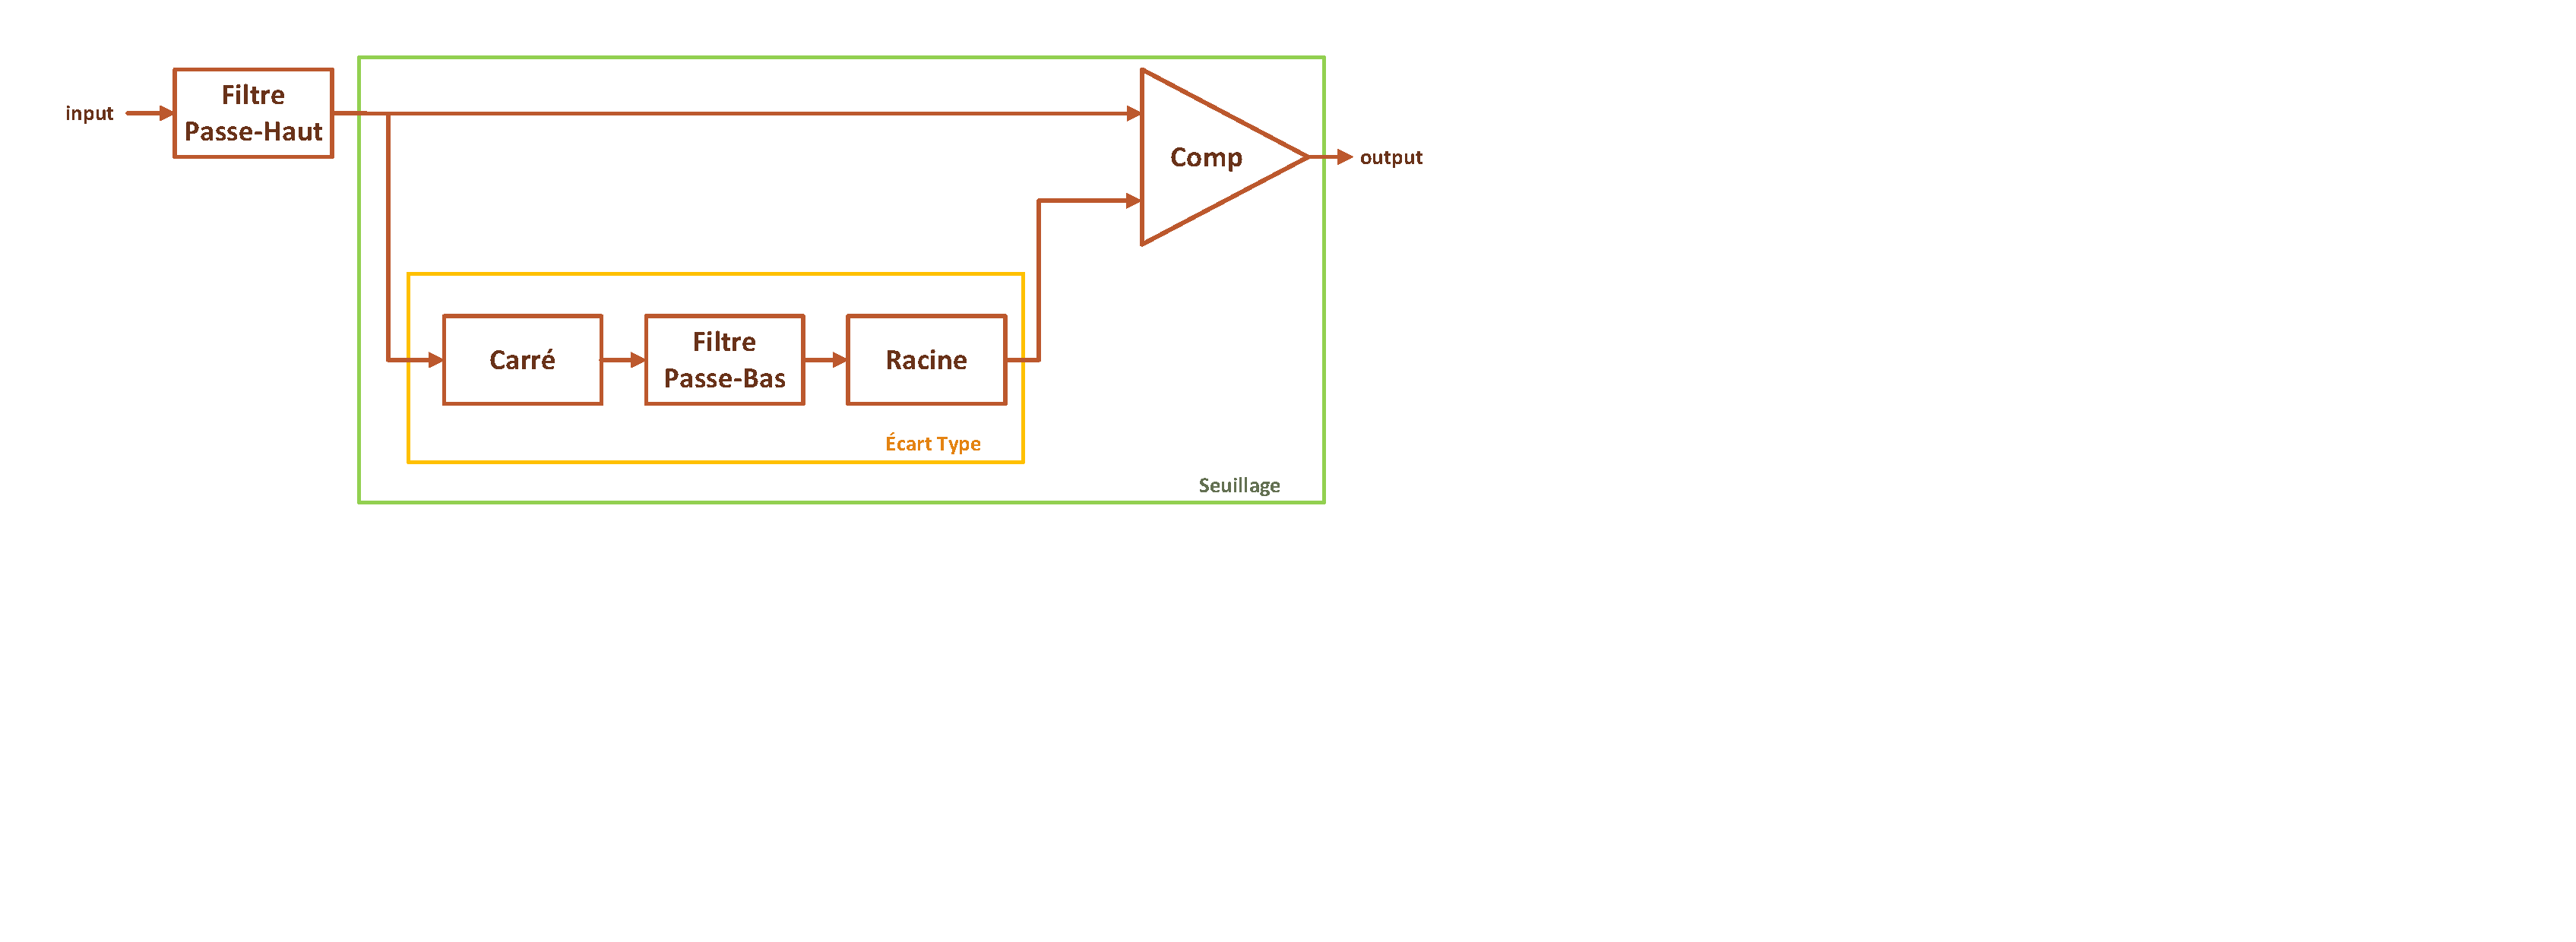
\includegraphics[width=\textwidth, keepaspectratio]{chainXavier.pdf}
\caption{Schéma de principe du calcul de l'écart type}
\end{figure}
\end{itemize}
\end{itemize}
\newpage
\section{Implémentation depuis le SystemC}
Les schémas présentés en Figures X et X permettent de se représenter le fonctionnement de la chaîne globale. La modularité du SystemC nous permet alors de concevoir une paire de fichiers, un fichier source de description ainsi qu'un \textit{header}, pour chacun des blocs composant ces schémas. Il convient de détailler le cheminement suivi à partir de la création de ces fichiers jusqu'à leur implémentation sur la carte Nexys 4. Cette partie vient donc présenter le flot de conception/compilation lié au SystemC et sa mise en oeuvre lors du projet.

\subsection{Flot de compilation}
L'apprentissage d'un nouveau langage de description ou de programmation passe nécessairement par la compréhension du flot de compilation qui lui est associé. Pour le SystemC, on peut découper ce flot en quatre étapes principales illustrées par la Figure X :
\begin{figure}[H]
\centering
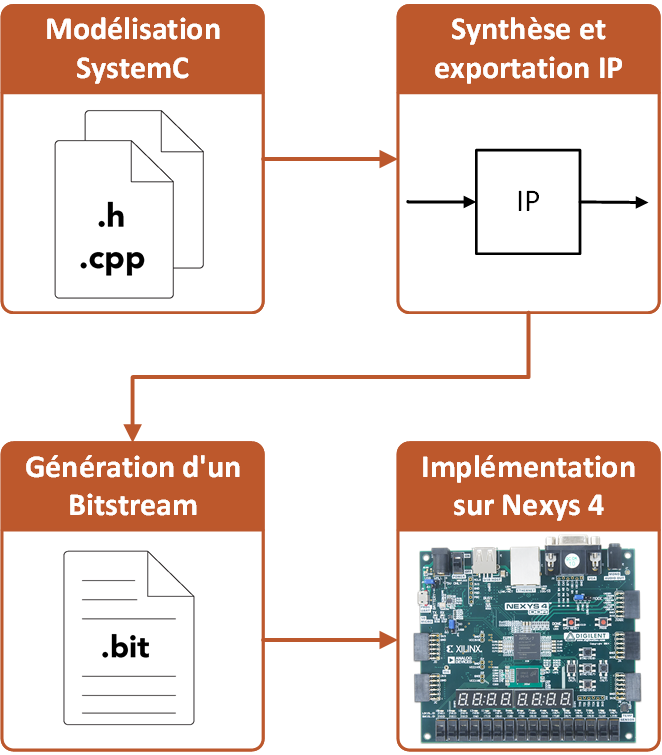
\includegraphics[scale=0.5, keepaspectratio]{Dessin2.png}
\caption{Flot de compilation}
\end{figure}
\begin{itemize}
\item[\textbullet] \textbf{Modélisation SystemC} : dans un premier temps il convient de décrire en SystemC le système que l'on souhaite modéliser. Pour cela, on rédige des fichiers sources \sout{dans un IDE} SystemC pour symboliser chacun des blocs décrits précédemment. \\
\item[\textbullet] \textbf{Synthèse et exportation IP} : une fois les fichiers SystemC écrits, on peut désormais les passer dans l'environnement \textit{Vivado HLS} afin de les synthéthiser et d'exporter un ou plusieurs blocs sous forme d'IP (\textit{Intellectual Property}). Ces blocs IP sont des blocs logiques, avec des entrées et des sorties, qui vont être implémentés sur FPGA par la suite. \\
\item[\textbullet] \textbf{Génération d'un Bitsream} : un bloc IP ne pouvant être envoyé directement sur FPGA, il convient de l'intégrer dans un \textit{top-level}, décrit en langage VHDL, pour pouvoir notamment interfacer ses entrées et sorties avec les entrées et sorties physiques de la carte Nexys 4. Pour ce faire, l'environnement \textit{Vivado} est requis et permet de générer un \textit{bitsream} d'extension \texttt{.bit}. \\
\item[\textbullet] \textbf{Implémentation sur Nexys 4} : finalement, le \textit{bitsream} peut être envoyé sur la carte cible, dans notre cas la carte Nexys 4, via le port série de notre ordinateur. A ce stade, les fichiers décrits en SystemC sont implémentés sur FPGA.\\
\end{itemize}
Le flot de compilation présenté ici allie le développement \textit{software} de sources SystemC, et l'implémentation \textit{hardware} des blocs ainsi créés. Il s'agit là du flot de compilation suivi lors du projet et les parties 2.2 et 2.3 suivantes viennent détailler sa mise en pratique.


\subsection{Modélisation en SystemC et simulations}
En premier lieu, le SystemC possède de nombreux outils permettant la description de modules au même titre qu'un langage de bas niveau tel que le VHDL :\\

\begin{itemize}
\item[•] La classe \texttt{sc\_module} peut facilement être assimilé à une \texttt{entity} en VHDL, tandis que sa nature de classe lui permet d'utiliser des outils de C++ tel qu'un constructeur, \texttt{sc\_ctor}.
\item[•] Les processus séquentiel et combinatoire sont quant à eux modélisés respectivement par des méthodes \texttt{sc\_cthread}/\texttt{sc\_thread} et \texttt{sc\_method}.
\item[•] Enfin le type de donnée \texttt{sc\_int} permet la modélisation des signaux logiques \texttt{std\_logic}.\\
\end{itemize}

Cependant, le réel interêt d'utiliser le langage SystemC afin de décrire nos sources repose sur la flexibilité apportée par l'utilisation d'un langage de haut niveau, comme par exemple l'utilisation de constructeur comme souligné pus tôt.

\begin{itemize}
\item[•] \textbf{La classe \texttt{sc\_fifo}} :\\
En effet, l'une des tâches qui demande le plus rigueur lors de la description d'un système \textit{hardware}, est la synchronisation de l'ensemble des modules. Celle-ci peut passer à travers la mise en place d'une machine d'états ou encore par la transmission de signaux de contrôle ou de validation entre chaque modules. La classe \texttt{sc\_fifo} est une classe synchrone qui instancie un tableau de donné, du type souhaité. L'utilisation de \textit{fifo} de taille infinie nous a permit de décrire nos modules indépendament les uns des autres, sans se soucier de la synchronisation et donc de l'idée d'horloge. En effet, les méthodes \texttt{read} et \texttt{write} de la classe \texttt{sc\_fifo} sont bloquantes, c'est à dire que les différents modules seront automatiquement en attente en cas d'absence de données par exemple.\\

\item[•] \textbf{Le type \textit{float}} :\\
Un autre avantage offert par l'utilisation d'un langage de haut niveau, est la possibilité de manipulé des \textit{float}. Malgré le fort coût matériel à l'implémentation, ce type données nous permet de mettre en place des calculs bien plus simplement en comparaison avec des calculs sur virgule fixe, bien souvent nécessaire lors d'une description VHDL.\\
\end{itemize}

Une fois les modules décris en SystemC, l'ensemble de la chaîne peut être instancié à l'image d'un \textit{top level} en VHDL. De nombreuses simulations on été effectuées afin de valider la bon fonctionnment de la chaîne. Pour ce faire, des modules de sauvegarde de données dans des fichiers textes ont été insérés entre chaque bloc du système. Ainsi ils nous a été possible de rapidement mettre à jour des erreurs de comportement. L'architecture des différents blocs décrits en SystemC étant très similaire, une \textit{fifo} \texttt{sc\_fifo<float>} en entrée et en sortie, l'étape de simulation s'en est trouvée facilité.

\begin{figure}[H]
\centering
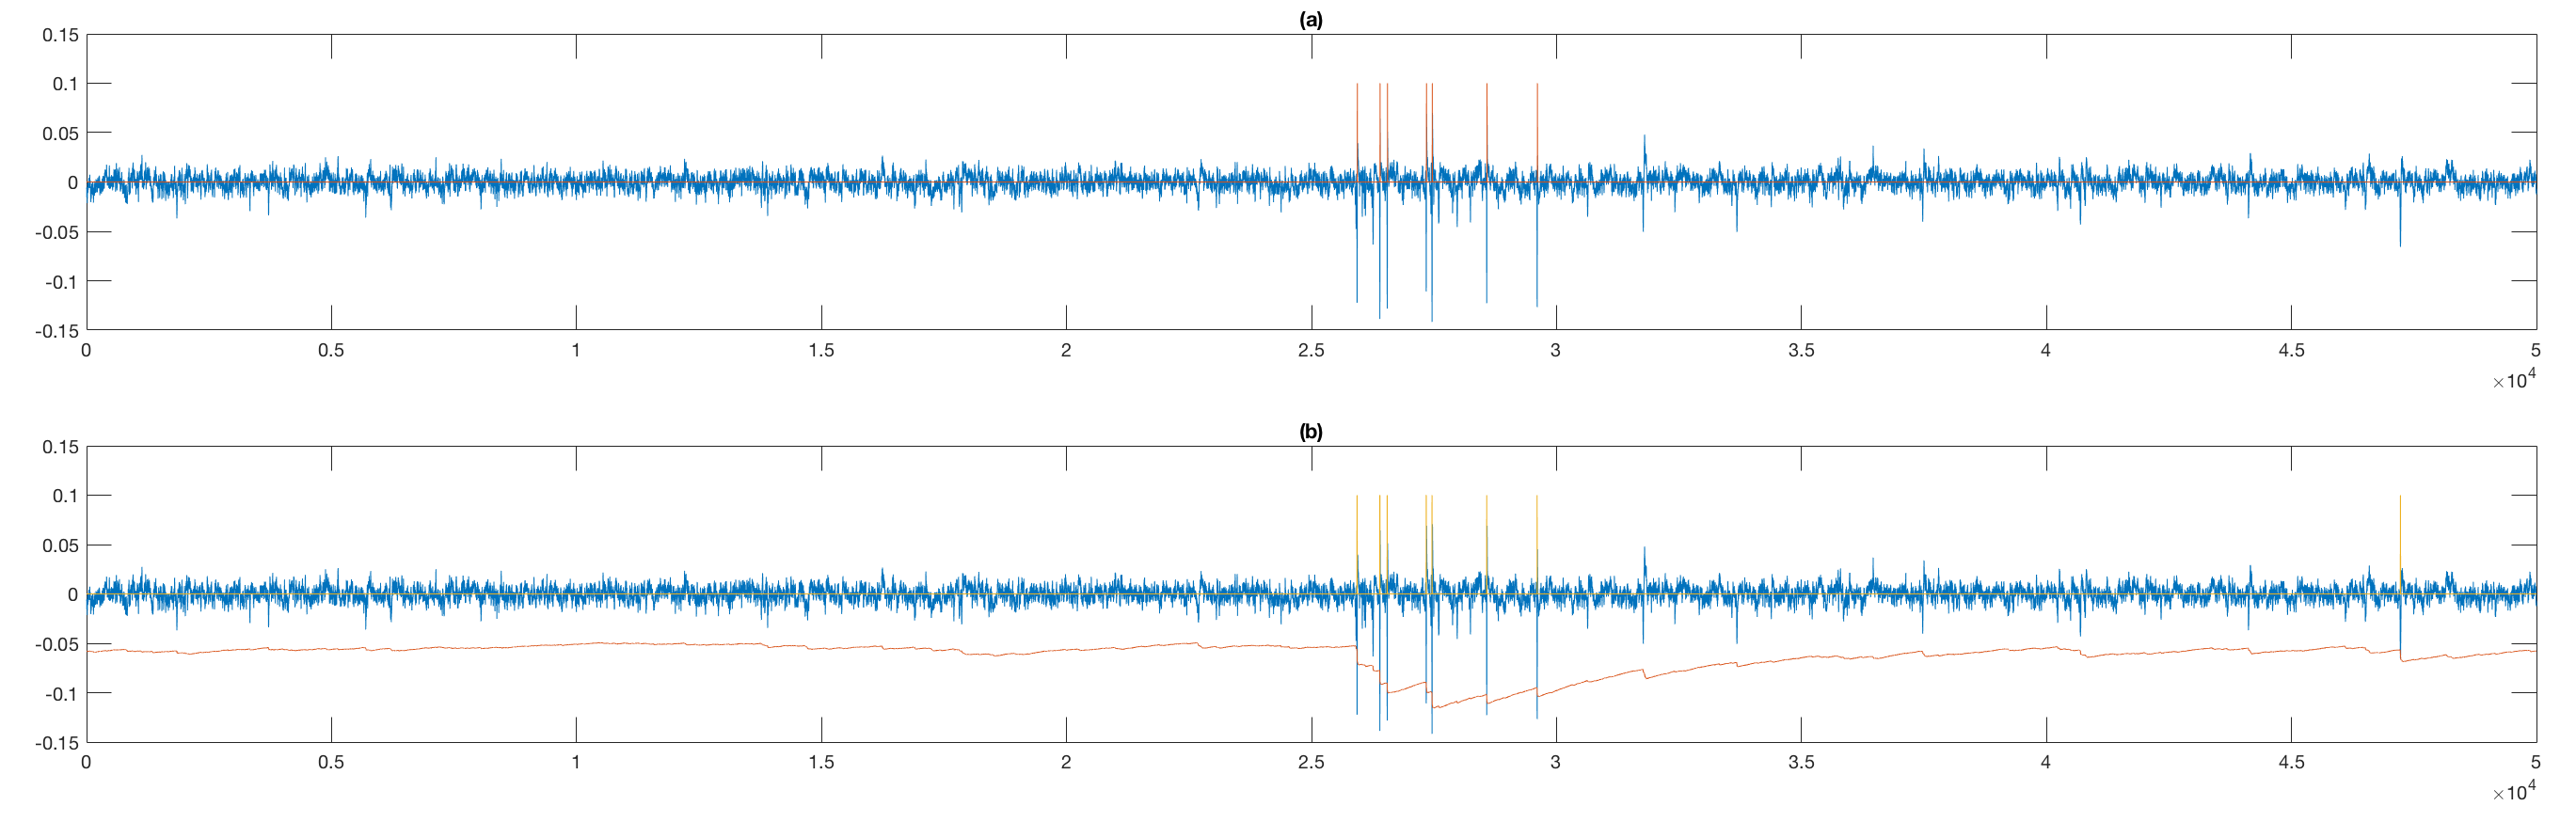
\includegraphics[scale =0.18, keepaspectratio]{results.png}
\caption{Mise en parallèle avec les résultats de Yannick Bornat}
\end{figure}
La figure 7 illustre ce bon fonctionnment, en a) on peut voir les pics détecter par le module VHDL de Yannick Bornat et en b) les pics détecter à l'aide de notre module de seuillage.
\subsection{Implémentation sur FPGA et validation}
Une fois les fichiers SystemC écrits et les simulations en \textit{software} vérifiées, il convient de tester les blocs et chaînes entières en \textit{hardware}. Pour cela, un environnement de test a été mis en place et il est illustré en Figure X.
\begin{figure}[H]
\centering
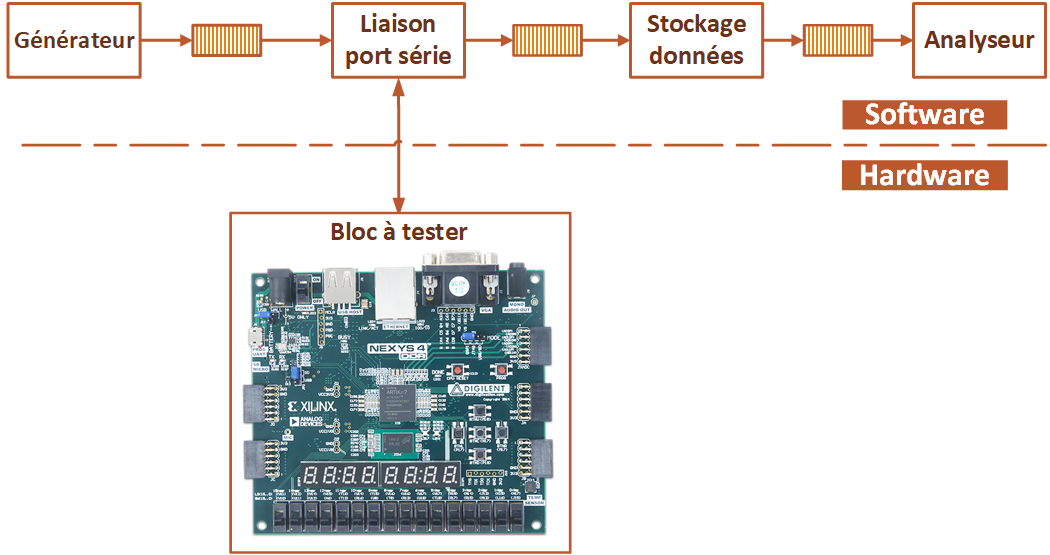
\includegraphics[width=\textwidth, keepaspectratio]{Dessin6.png}
\caption{Environnement de test}
\end{figure}
\noindent On distingue ici deux parties essentielles :\\
\begin{itemize}
\item[\textbullet] la partie \textit{software} : elle se déroule sur un ordinateur, sous \textit{Vivado HLS} par exemple, et permet de lancer une simulation,\\
\item[\textbullet] la partie \textit{hardware} : elle représente la carte Nexys 4 reliée en USB sur le port série de l'ordinateur, elle contient également l'implémentation du bloc IP à tester.\\
\end{itemize} 

Avant de tester les chaînes globales développées en SystemC, les blocs réalisant la racine carrée ainsi que la puissance au carré ont notamment été implémentés sur FPGA. Pour ce faire, le bloc "\textit{Générateur}" permet de venir lire les données d'entrée stockées dans un fichier texte, que ce soit les valeurs extraites du signal biomédical ou bien des valeurs plus rudimentaires pour tester seulement un bloc. Après passage dans une FIFO, les données sont envoyées sur le port série et traitées sur le FPGA. Ce dernier contient l'IP que l'on souhaite tester en \textit{hardware}, la racine carrée par exemple, et renvoie les données sortantes vers le bloc "\textit{Stockage données}". Ce bloc écrit alors les données calculées sur le FPGA dans un fichier texte. Comme expliqué en 2.2, les données contenues dans une FIFO doivent être consommées, c'est pourquoi le bloc "\textit{Analyseur}" se contente de venir lire dans la FIFO, pour fermer la chaîne de test. Cet environnement de test peut ainsi s'adapter à tout bloc qui compose notre chaîne globale et dont on souhaite vérifier le bon fonctionnement. \\ \\
\indent En ce qui concerne l'échange de données entre la partie \textit{software} et le FPGA, le module de communication utilisant l'UART et développé par Yannick Bornat a été utilisé. Cependant, les deux chaînes précédemment décrites manipulent des données de type \textit{float}, donc sur 32 bits, tandis que l'UART ne reçoit et renvoie que des données sur 8 bits. Pour palier à cette incompatibilité, des \textit{wrappers} ont été décrit en SystemC selon le modèle présenté en Figure X. Le \textit{wrapper} IN reçoit les données provenant de l'UART sur 8 bits et les reforme sur 32 bits, en attendant donc quatre paquets de 8 bits, et les envoie ensuite au bloc de test, tandis que le \textit{wrapper} OUT fait l'opération inverse et découpe la donnée en quatre paquets de 8 bits, chacun d'eux envoyé à l'UART. De plus, le bloc "\textit{Ouverture port série}" réalise également ce découpage des données sur 8 bits en entrée et la reformation de la donnée de sortie sur 32 bits car il communique directement avec l'UART et la partie \textit{software}. Ces deux wrappers ont alors été synthéthisés et exportés en tant qu'IP avec le bloc à tester.  
\begin{figure}[H]
\centering
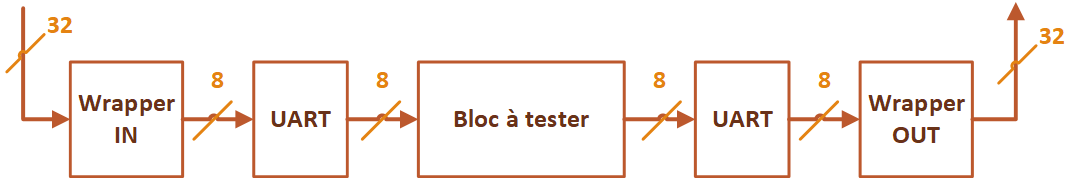
\includegraphics[width=\textwidth]{Dessin7.png}
\caption{UART Wrappers}
\end{figure}   

Lorsque les différents blocs ont été validés un à un sur cet environnement de test, les deux chaînes ont pu successivement être implémentées sur FPGA. Leur validation est, quant à elle, passée par une comparaison entre les données traitées et celles de référence obtenues après développement en VHDL de Yannick Bornat. La principale difficulté de cette démarche d'implémentation \textit{hardware} résidait dans l'envoi et la réception des données entre la chaîne de simulation et la carte Nexys 4. En effet, le goulot d'étranglement se trouve dans la communication avec l'UART qui attend de recevoir une donnée avant d'en transmettre une autre. Cet aspect-là est notamment dû à la manière dont nous avons écrit nos sources mais une fois cette notion appréhendée il a été possible de vérifier le fonctionnement de n'importe quels blocs.
\newpage
\section{Résultats}
Après simulation et implémentation de l'ensemble des blocs et de la chaine de filtrage, il est nécessaire de comparer les sorties afin de vérifier la similitude des deux systèmes et en noter les différences.
\subsection{Comparaison des sorties}
À l'aide d'un code sous Matlab, la sortie du système simulé est comparée aux données fournies par monsieur Bornat.L'idée ici est de mettre en avant le bon fonctionnement du système en montrant l'équivalence des résultats de sortie avec ceux du système de référence.Les indices des pics détectés sont donc extraits d'un fichier texte contenant les sorties du système et comparé avec les indices contenus dans le fichier de référence.La différence entre les indices sources et références est enregistrée et si celui-ci dépasse les 50 échantillons, la sortie source sera considérée comme une erreur. 
\begin{figure}[H]
	\centering
	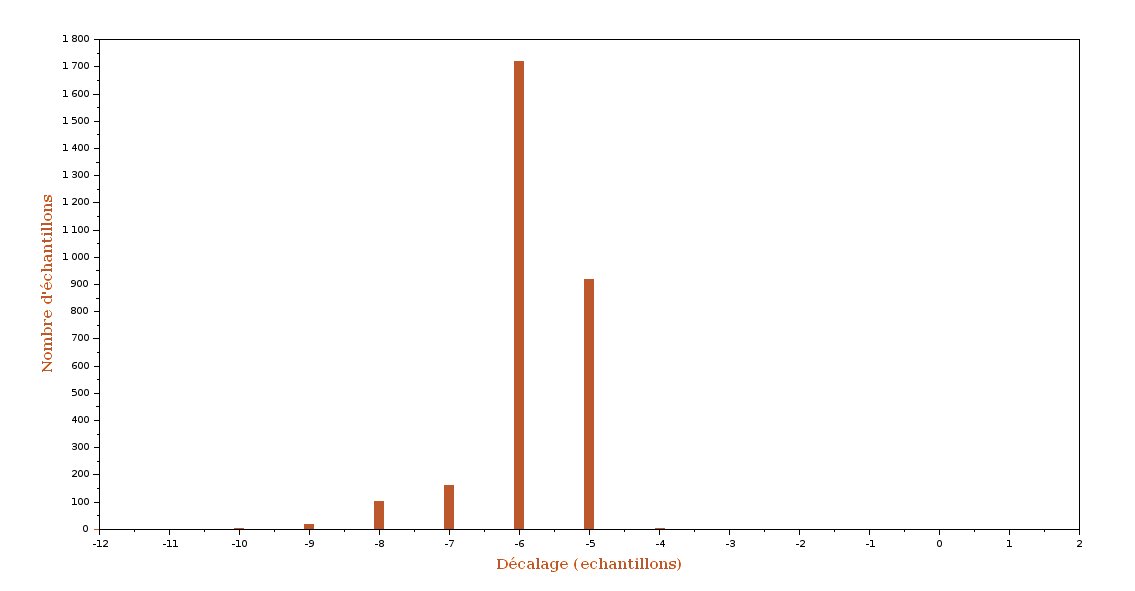
\includegraphics[scale=0.3, keepaspectratio]{ResultatSim.png}
	\caption{\textit{Représentation du décalage de détéction entre le système simulé et la référence}}
\end{figure}
La figure X montre les décalages retrouvés sur l'ensemble des pics fournis dans le fichier source. Le système montre 65 erreurs sur les 2990 pics ce qui correspond à un ratio $98 \%$ de similitude.Enfin, comme le montre la figure, les pics sont détectée entre 4 et 9 échantillons avant l'indice présent dans le fichier de référence. Ceci s'expliquait par une différence de moyen de détection entre la source et le système de référence.En effet, le pic biologique étant plus large qu'un simple échantillon, l'absence du système anti-rebond dans notre simulation explique parfaitement ce décalage.Nous avons donc considéré que les deux systèmes étaient équivalents en matière de comportement.
\newpage
\subsection{Ressources utilisées}
Après avoir validé le comportement de notre chaine, l'important maintenant est de comparer l'utilisation des ressources à l'aide du rapport de synthèse fourni par HLS.Cette comparaison est faite sans utiliser de moyen d'optimisation afin de juger des performances du systemC. Néanmoins, il va de soi que les performances d'un système écrit par des étudiants seront nettement moins bonnes que celles obtenues sur un système écrit par un utilisateur expérimenté du VHDL.
\begin{table}[h]
	\centering
	\begin{tabular}{|
	>{\columncolor[HTML]{F2B25C}}c |
	>{\columncolor[HTML]{FFFFFF}}r |
	>{\columncolor[HTML]{FFFFFF}}r |
	>{\columncolor[HTML]{FFFFFF}}c |}
	\hline
	\cellcolor[HTML]{BD591C} & \multicolumn{1}{c|}{\cellcolor[HTML]{F2B25C}SystemC (64 channels)} & \multicolumn{1}{c|}{\cellcolor[HTML]{F2B25C}VHDL} & \cellcolor[HTML]{F2B25C}Difference \\ \hline
	LUT                      & 5632                                                               & X                                                 & {\color[HTML]{CB0000} XXX}         \\ \hline
	DSP                      & 26                                                                 & 1                                                 & {\color[HTML]{CB0000} +2500\%}     \\ \hline
	FF                       & 2789                                                               & X                                                 & {\color[HTML]{CB0000} XXX}         \\ \hline
	RAM (512*32bits)         & 5                                                                  & 2                                                 & {\color[HTML]{CB0000} +150\%}      \\ \hline
	Development Time (hours) & 35                                                                 & 50                                                & {\color[HTML]{009901} -30\%}       \\ \hline
	\end{tabular}
	\caption{Utilisation des ressources des deux systèmes}
	\end{table}
	La table XX récapitule l'utilisation des ressources fournies pour notre système par HLS et par monsieur Bornat pour le sien. N'ayant pas senti l'utilité de s'intéresser au LUT et aux bascules flip-flop, ces données ne nous ont pas été communiquées.
	Il y a trois points intéressants dans ce tableau :
\begin{itemize}
	\item[•] \textbf{Le nombre de DSP} utilisés est nettement plus élevés. Cette différence s'explique par l'utilisation de nombres flottants sur 32 bits contre des nombres à virgule fixe sur 16 bits dans le système de référence. De plus, l'utilisation d'un seul DSP dans le système de référence montre la volonté de monsieur Bornat de limiter le nombre de DSP utilisés ce qui n'a pas été notre cas.
	\item[•] \textbf{Le nombre de RAM} utilisées qui découlent de l'allocation par HLS d'un bloc RAM pour chaque tableau présent dans notre code. Une fois de plus, cette valeur se trouve être plus élevée que celle du système de référence.
	\item[•] \textbf{Le temps de développement} quant à lui est $30\%$ inférieur dans le cadre d'un développement en systemC par rapport à une description en VHDL.
\end{itemize}
Ces données nous montrent que l'utilisation du systemC via HLS pour la synthèse de systèmes permet un gain de temps non négligeable. L'optimisation des ressources est quant à elle possible en ajoutant simplement quelques directives pour la synthèse et n'a pas été traité ici. 
\newpage
\section{Conclusion}

\end{document}


